% !LW recipe=pdflatex
\documentclass{standalone}

\usepackage{animate}
\usepackage{amsmath, amssymb, amsthm, mathrsfs, amsfonts, dsfont}
\usepackage{ascmac}
\usepackage{bbm}
\usepackage{bm}
\usepackage{breakcites}
\usepackage{calc}
\usepackage{enumerate}
\usepackage{ifthen}
\usepackage{mathtools}
\usepackage{makecell}
\usepackage{mlmodern}
\usepackage{newtxtext}
\usepackage{optidef}
\usepackage{physics}
\usepackage{pifont}
\usepackage{setspace}
\usepackage{stfloats}
\usepackage{subcaption}
\usepackage{svg}
\usepackage{tikz}
\usepackage{xparse}
\usepackage[all]{xy}

\usepackage{float}
\usepackage{color}
\usepackage{graphicx}
\usepackage[colorlinks=true, allcolors=blue]{hyperref}


% === Commands ===

\definecolor{cA}{HTML}{0072BD}
\definecolor{cB}{HTML}{EDB120}
\definecolor{cC}{HTML}{77AC30}
\definecolor{cD}{HTML}{D95319}
\definecolor{cE}{HTML}{7E2F8E}
\newcommand{\cAText}[1]{\textcolor{cA}{#1}}
\newcommand{\cBText}[1]{\textcolor{cB}{#1}}
\newcommand{\cCText}[1]{\textcolor{cC}{#1}}
\newcommand{\cDText}[1]{\textcolor{cD}{#1}}
\newcommand{\cEText}[1]{\textcolor{cE}{#1}}
\newcommand{\red}[1]{\textcolor{red}{#1}}
\newcommand{\blue}[1]{\textcolor{blue}{#1}}
\newcommand{\green}[1]{\textcolor{green}{#1}}
\newcommand{\gray}[1]{\textcolor{gray}{#1}}
\newcommand{\black}[1]{\textcolor{black}{#1}}

\newcommand{\st}{\text{ s.t. }}
\newcommand{\Img}[1]{\mathrm{Im}\qty(#1)}
\newcommand{\Ker}[1]{\mathrm{Ker}\qty(#1)}
\newcommand{\Supp}[1]{\mathrm{supp}\qty(#1)}
\newcommand{\Rank}[1]{\mathrm{rank}\qty(#1)}
\newcommand{\floor}[1]{\left\lfloor #1 \right\rfloor}
\newcommand{\ceil}[1]{\left\lceil #1 \right\rceil}
% C++ (https://tex.stackexchange.com/questions/4302/prettiest-way-to-typeset-c-cplusplus)
\newcommand{\Cpp}{C\nolinebreak[4]\hspace{-.05em}\raisebox{.4ex}{\relsize{-3}{\textbf{++}}}}
% https://tex.stackexchange.com/questions/28836/typesetting-the-define-equals-symbol
\newcommand{\defeq}{\coloneqq}
\newcommand{\eqdef}{\eqqcolon}
% https://tex.stackexchange.com/questions/5502/how-to-get-a-mid-binary-relation-that-grows
\newcommand{\relmiddle}[1]{\mathrel{}\middle#1\mathrel{}}
\newcommand{\cmark}{\cCText{\ding{51}}} % check mark
\newcommand{\xmark}{\cDText{\ding{55}}} % cross mark

\DeclareMathOperator{\Proj}{Proj}
\DeclareMathOperator{\Exp}{Exp}
\DeclareMathOperator{\Hess}{Hess}
\DeclareMathOperator{\Retr}{Retr}
\DeclareMathOperator{\Span}{span}
\DeclareMathOperator{\myGrad}{grad}
\renewcommand{\grad}{\myGrad}

% https://tex.stackexchange.com/questions/564216/newcommand-for-each-letter
\ExplSyntaxOn
\NewDocumentCommand{\definealphabet}{mmmm}{
\int_step_inline:nnn{`#3}{`#4}{
\cs_new_protected:cpx{#1 \char_generate:nn{##1}{11}}{
\exp_not:N #2{\char_generate:nn{##1}{11}}}}}
\ExplSyntaxOff

\definealphabet{bb}{\mathbb}{A}{Z}
\definealphabet{rm}{\mathrm}{A}{Z}
\definealphabet{cal}{\mathcal}{A}{Z}
% \definealphabet{scr}{\mathscr}{A}{Z}
\definealphabet{frak}{\mathfrak}{a}{z}
\definealphabet{frak}{\mathfrak}{A}{Z}

% === Settings ===

% https://qiita.com/rityo_masu/items/efd44bc8f9229e014237
\allowdisplaybreaks[4]

\usetikzlibrary{
  3d,
  fit,
  calc,
  math,
  matrix,
  patterns,
  backgrounds,
  arrows.meta,
  decorations.pathmorphing,
}

\begin{document}

\begin{tabular}{cccccc}
  \multicolumn{6}{c}{\large \textbf{\texttt{jagmesh8}} $(\abs{V}=1141, \abs{E}=3162, \text{density}=0.486\text{\%})$ \quad Figures are at 150 iterations.} \\
  \raisebox{-.5\height}{\includegraphics[width=0.55\columnwidth]{plot/jagmesh8_2.pdf}} &
  \makecell{\textsf{RAND-FR}\\[-0.2em]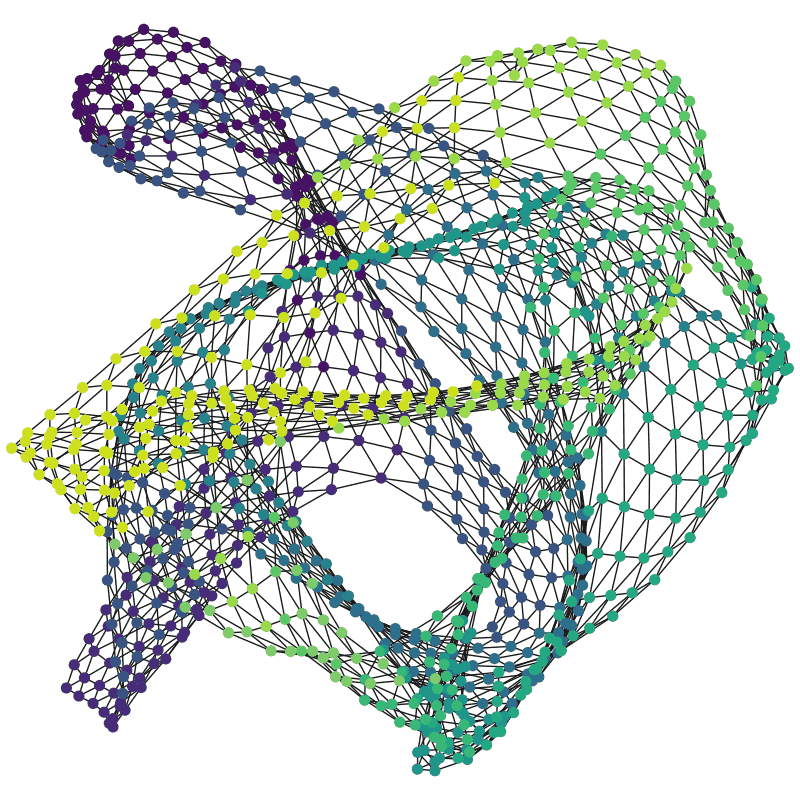
\includegraphics[width=0.27\columnwidth]{vis/jagmesh8_FR_2.png}} &
  \makecell{\textsf{\textbf{CN}-FR (proposed)}\\[-0.2em]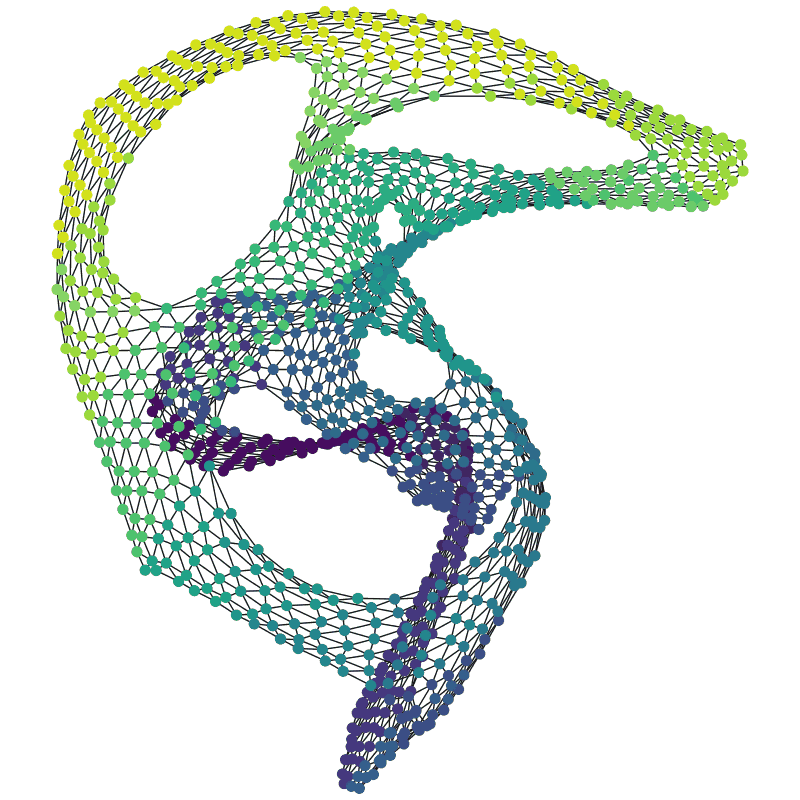
\includegraphics[width=0.27\columnwidth]{vis/jagmesh8_CN-FR_2.png}} &
  \makecell{\textsf{RAND-L-BFGS}\\[-0.2em]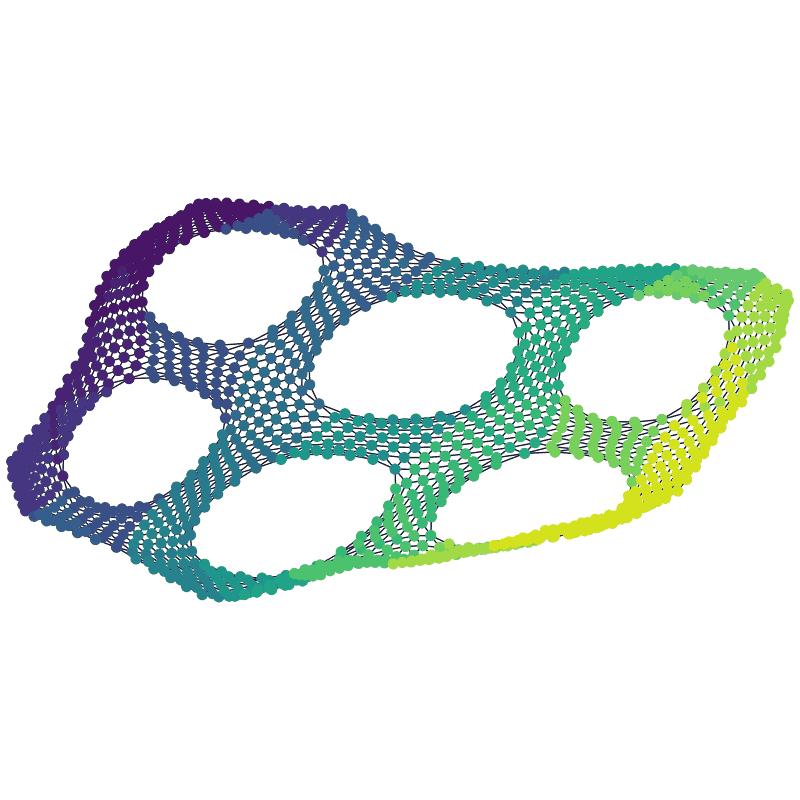
\includegraphics[width=0.27\columnwidth]{vis/jagmesh8_L-BFGS_2.png}} &
  \makecell{\textsf{\textbf{CN}-L-BFGS (proposed)}\\[-0.2em]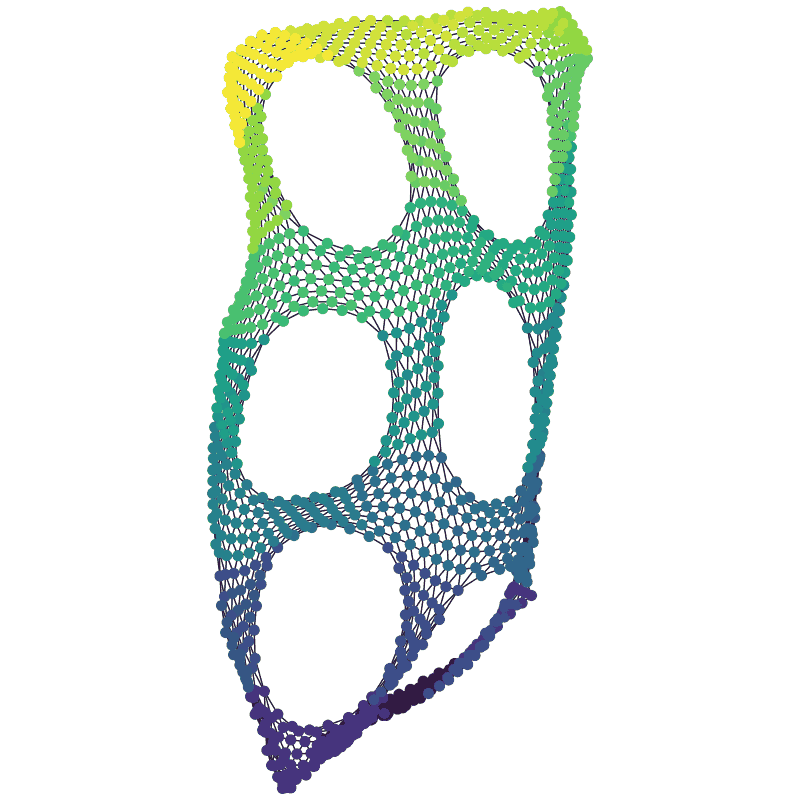
\includegraphics[width=0.27\columnwidth]{vis/jagmesh8_CN-L-BFGS_2.png}} &
  \makecell{\textsf{BEST}\\[-0.2em]\includegraphics[width=0.27\columnwidth]{vis/opt_jagmesh8_2.png}} \\

  \multicolumn{6}{c}{\large \textbf{\texttt{bcsstk14}} $(\abs{V}=1766, \abs{E}=30824, \text{density}=1.978\text{\%})$ \quad Figures are at 50 iterations.} \\
  \raisebox{-.5\height}{\includegraphics[width=0.55\columnwidth]{plot/bcsstk14_2.pdf}} &
  \makecell{\textsf{RAND-FR}\\[-0.2em]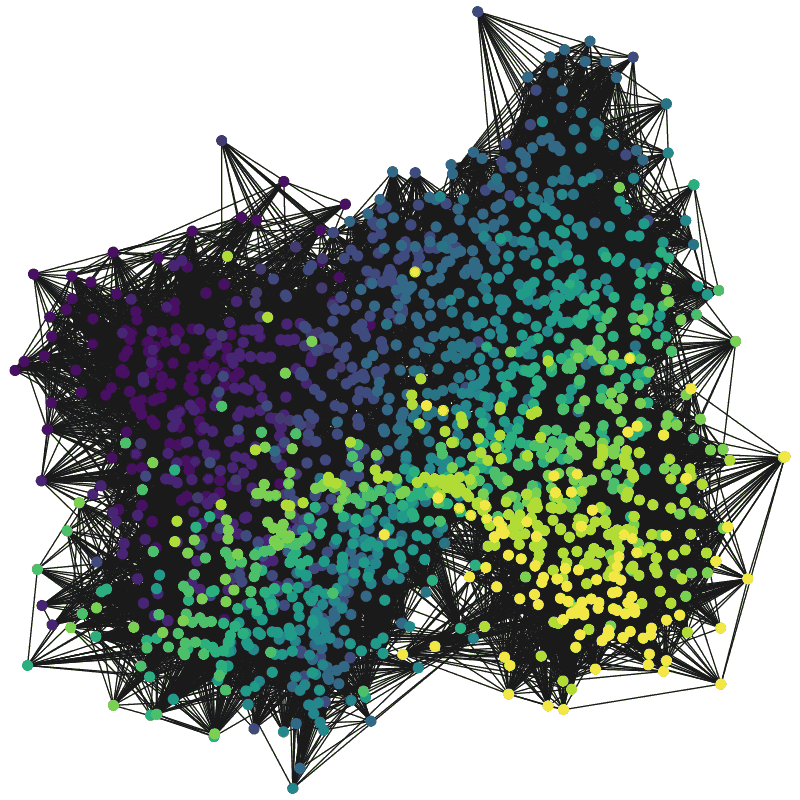
\includegraphics[width=0.27\columnwidth]{vis/bcsstk14_FR_2.png}} &
  \makecell{\textsf{\textbf{CN}-FR (proposed)}\\[-0.2em]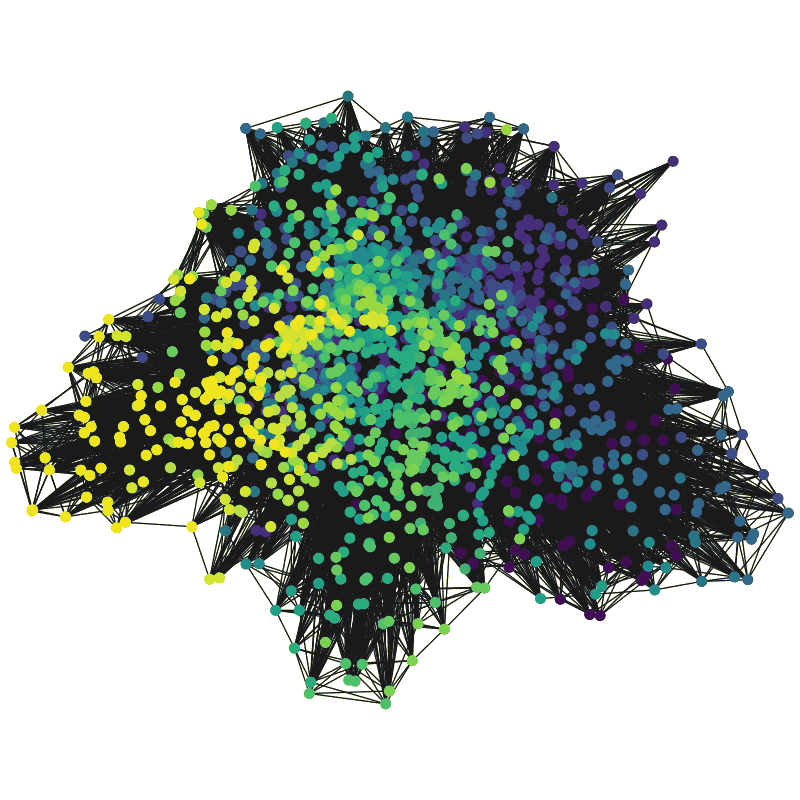
\includegraphics[width=0.27\columnwidth]{vis/bcsstk14_CN-FR_2.png}} &
  \makecell{\textsf{RAND-L-BFGS}\\[-0.2em]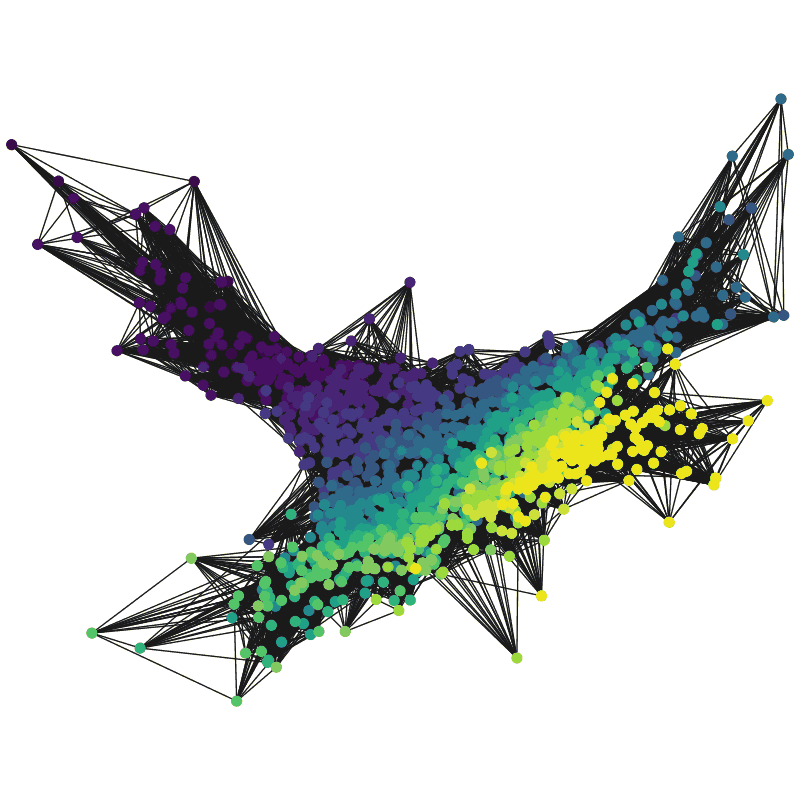
\includegraphics[width=0.27\columnwidth]{vis/bcsstk14_L-BFGS_2.png}} &
  \makecell{\textsf{\textbf{CN}-L-BFGS (proposed)}\\[-0.2em]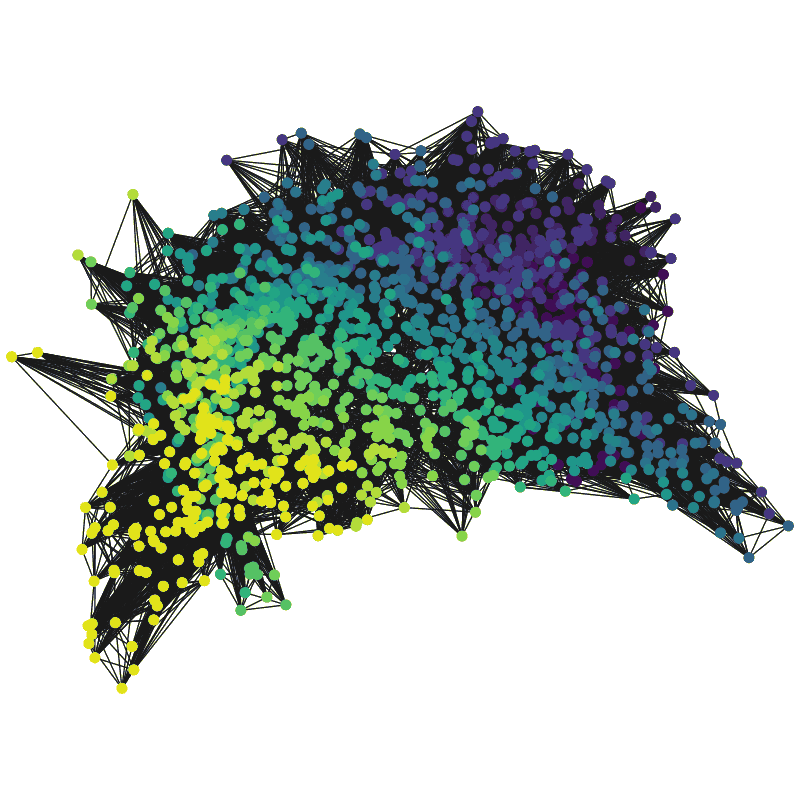
\includegraphics[width=0.27\columnwidth]{vis/bcsstk14_CN-L-BFGS_2.png}} &
  \makecell{\textsf{BEST}\\[-0.2em]\includegraphics[width=0.27\columnwidth]{vis/opt_bcsstk14_2.png}} \\

  \multicolumn{6}{c}{\large \textbf{\texttt{bcsstk15}} $(\abs{V}=3942, \abs{E}=56934, \text{density}=0.733\text{\%})$ \quad Figures are at 100 iterations.} \\
  \raisebox{-.5\height}{\includegraphics[width=0.55\columnwidth]{plot/bcsstk15_2.pdf}} &
  \makecell{\textsf{RAND-FR}\\[-0.2em]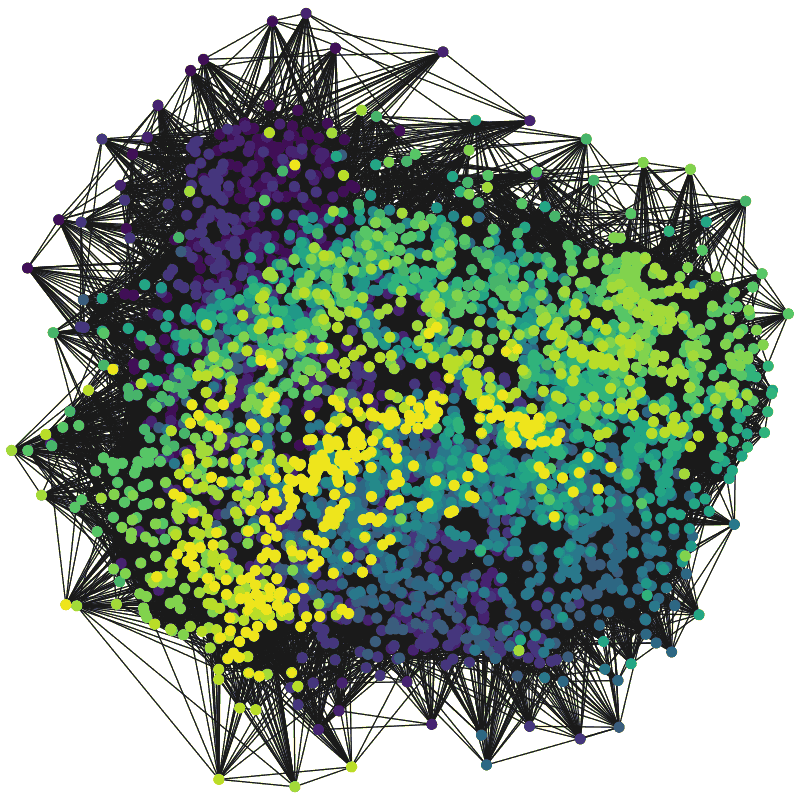
\includegraphics[width=0.27\columnwidth]{vis/bcsstk15_FR_2.png}} &
  \makecell{\textsf{\textbf{CN}-FR (proposed)}\\[-0.2em]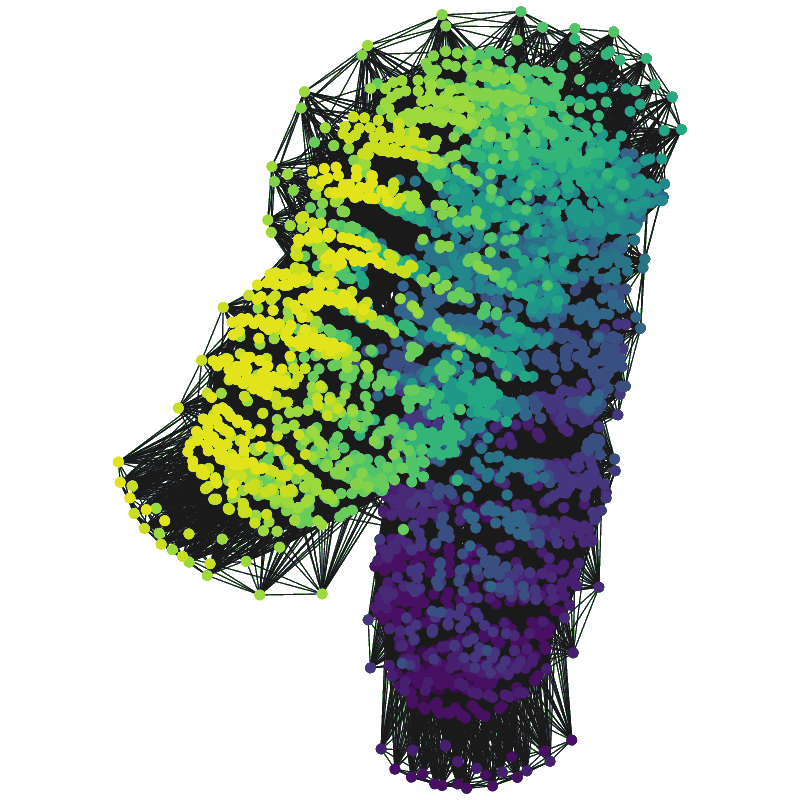
\includegraphics[width=0.27\columnwidth]{vis/bcsstk15_CN-FR_2.png}} &
  \makecell{\textsf{RAND-L-BFGS}\\[-0.2em]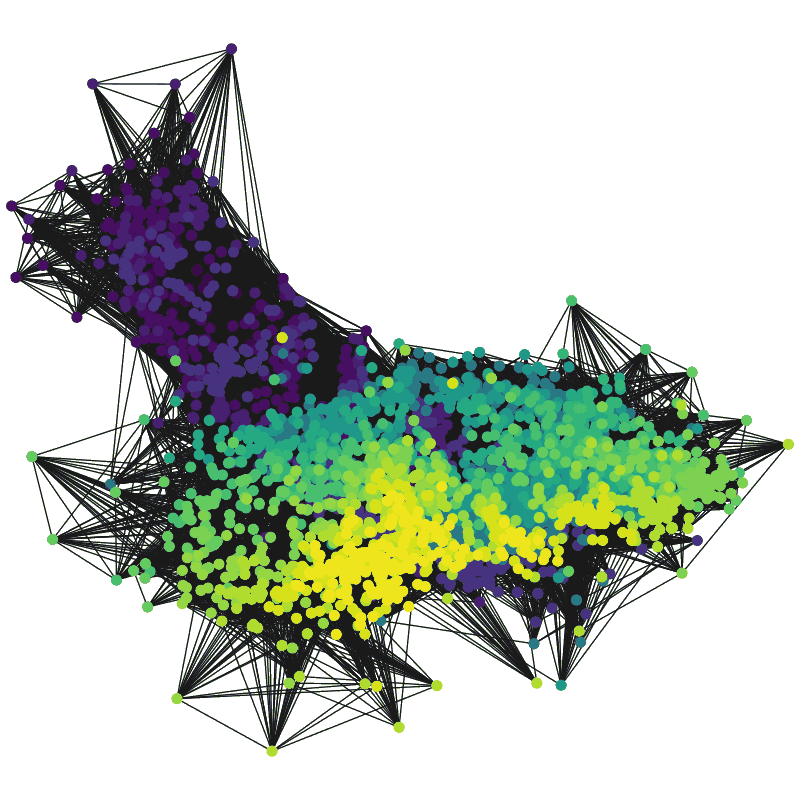
\includegraphics[width=0.27\columnwidth]{vis/bcsstk15_L-BFGS_2.png}} &
  \makecell{\textsf{\textbf{CN}-L-BFGS (proposed)}\\[-0.2em]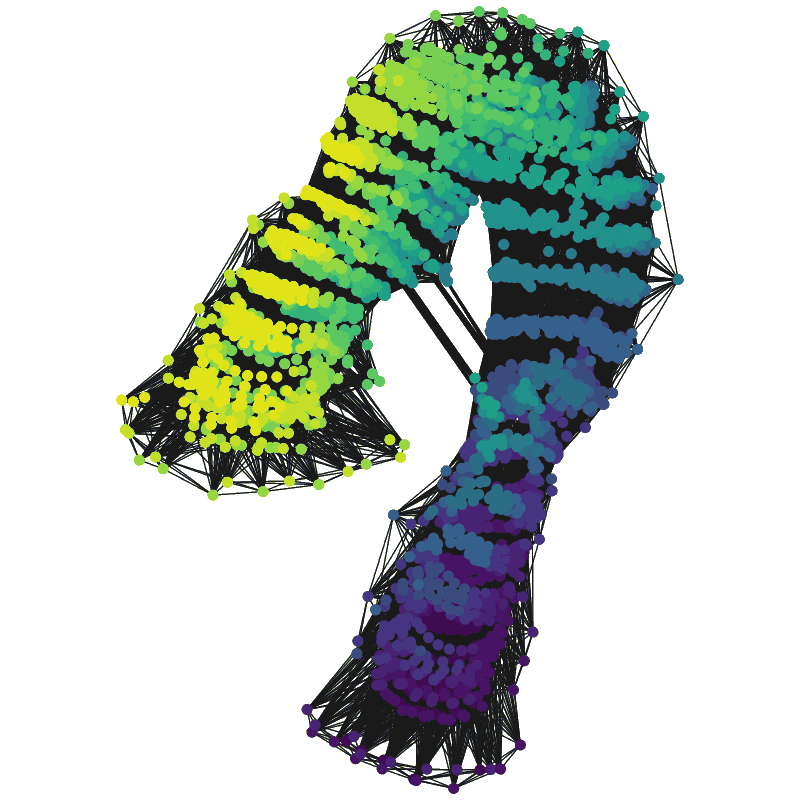
\includegraphics[width=0.27\columnwidth]{vis/bcsstk15_CN-L-BFGS_2.png}} &
  \makecell{\textsf{BEST}\\[-0.2em]\includegraphics[width=0.27\columnwidth]{vis/opt_bcsstk15_2.png}} \\

  \multicolumn{6}{c}{\large \textbf{\texttt{bcsstk16}} $(\abs{V}=4810, \abs{E}=142747, \text{density}=1.234\text{\%})$ \quad Figures are at 150 iterations.} \\
  \raisebox{-.5\height}{\includegraphics[width=0.55\columnwidth]{plot/bcsstk16_2.pdf}} &
  \makecell{\textsf{RAND-FR}\\[-0.2em]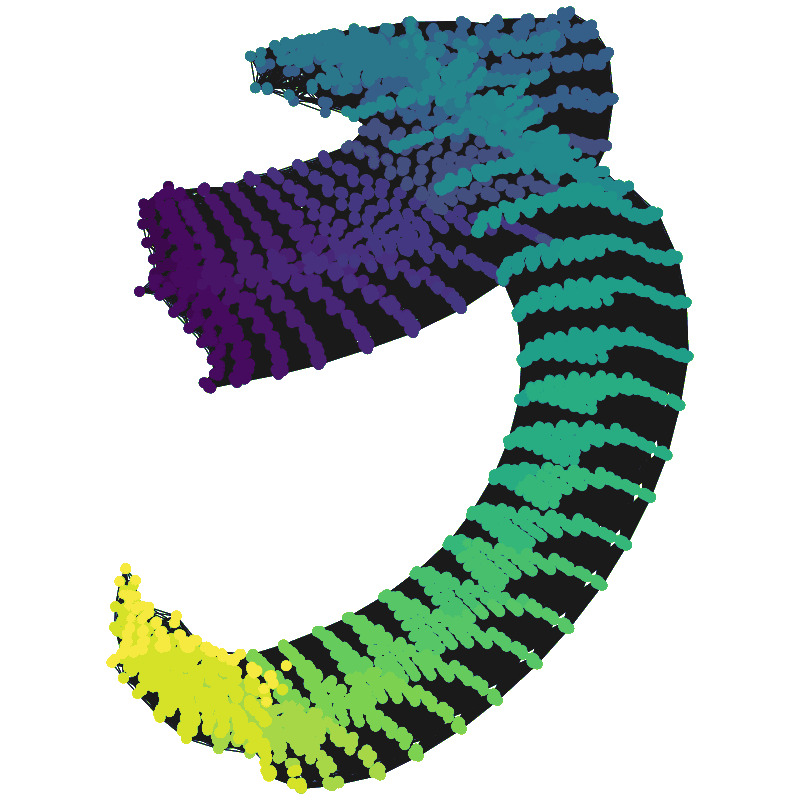
\includegraphics[width=0.27\columnwidth]{vis/bcsstk16_FR_2.png}} &
  \makecell{\textsf{\textbf{CN}-FR (proposed)}\\[-0.2em]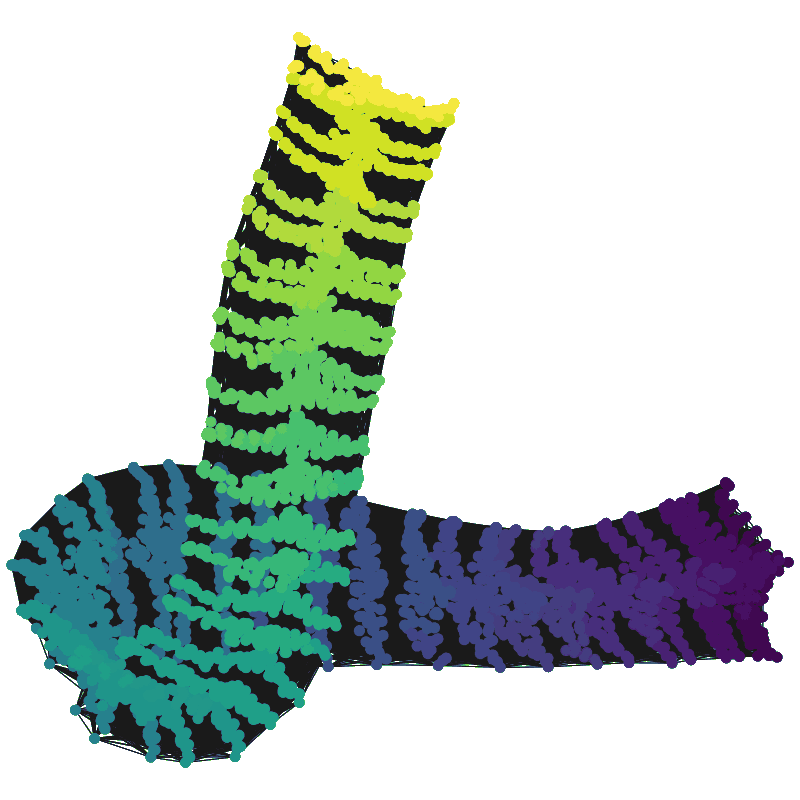
\includegraphics[width=0.27\columnwidth]{vis/bcsstk16_CN-FR_2.png}} &
  \makecell{\textsf{RAND-L-BFGS}\\[-0.2em]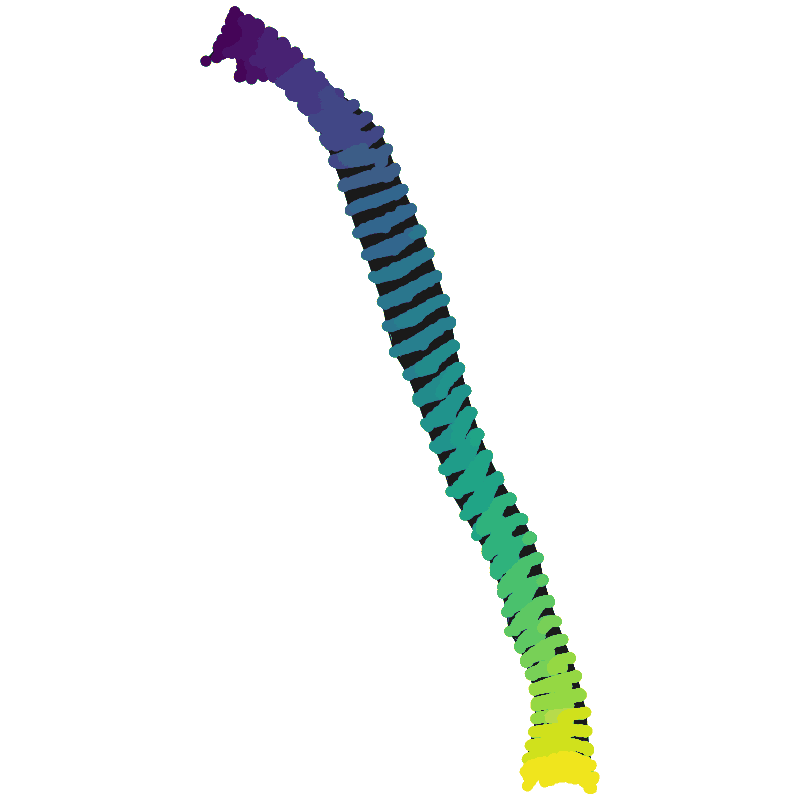
\includegraphics[width=0.27\columnwidth]{vis/bcsstk16_L-BFGS_2.png}} &
  \makecell{\textsf{\textbf{CN}-L-BFGS (proposed)}\\[-0.2em]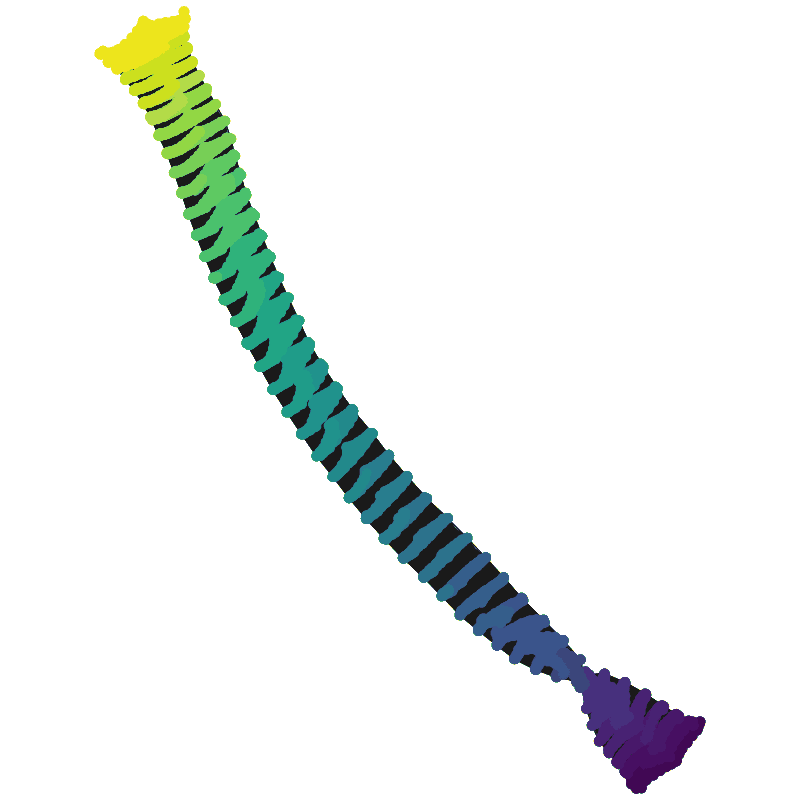
\includegraphics[width=0.27\columnwidth]{vis/bcsstk16_CN-L-BFGS_2.png}} &
  \makecell{\textsf{BEST}\\[-0.2em]\includegraphics[width=0.27\columnwidth]{vis/opt_bcsstk16_2.png}} \\

  \multicolumn{6}{c}{\large \textbf{\texttt{USpowerGrid}} $(\abs{V}=4941, \abs{E}=6594, \text{density}=0.054\text{\%})$ \quad Figures are at 150 iterations.} \\
  \raisebox{-.5\height}{\includegraphics[width=0.55\columnwidth]{plot/USpowerGrid_2.pdf}} &
  \makecell{\textsf{RAND-FR}\\[-0.2em]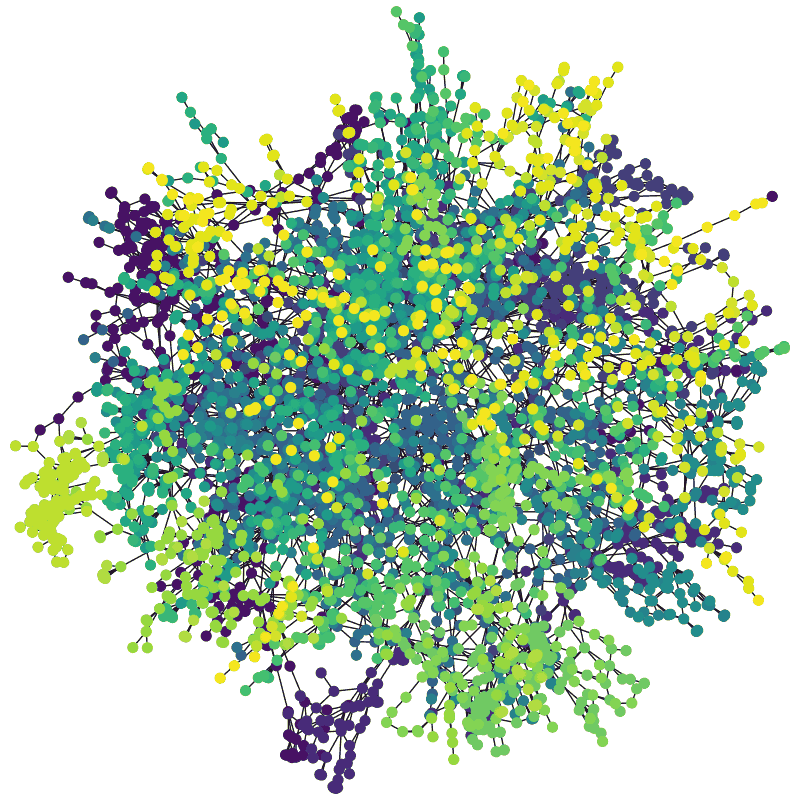
\includegraphics[width=0.27\columnwidth]{vis/USpowerGrid_FR_2.png}} &
  \makecell{\textsf{\textbf{CN}-FR (proposed)}\\[-0.2em]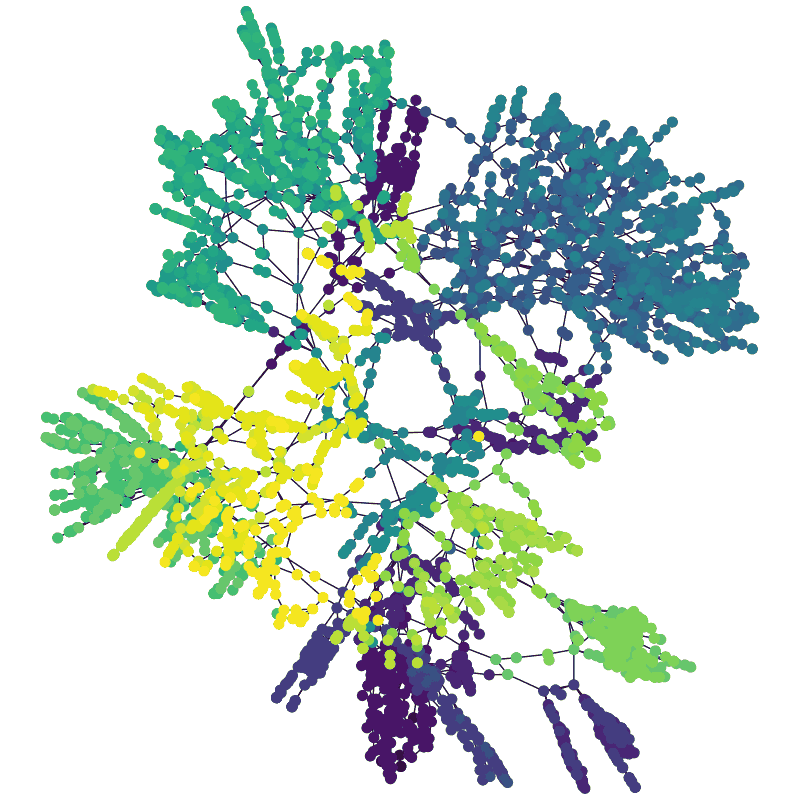
\includegraphics[width=0.27\columnwidth]{vis/USpowerGrid_CN-FR_2.png}} &
  \makecell{\textsf{RAND-L-BFGS}\\[-0.2em]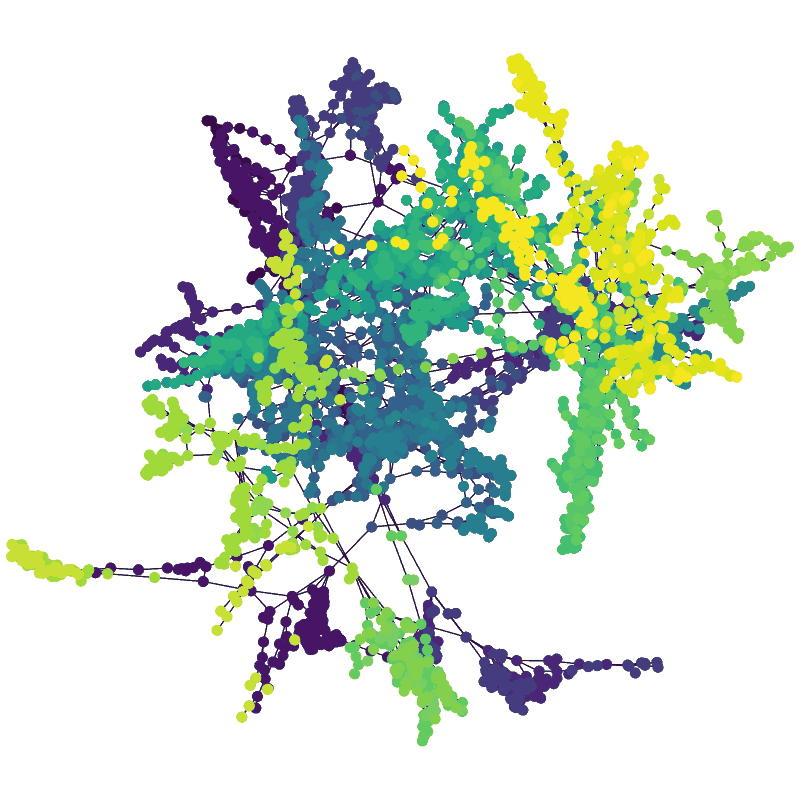
\includegraphics[width=0.27\columnwidth]{vis/USpowerGrid_L-BFGS_2.png}} &
  \makecell{\textsf{\textbf{CN}-L-BFGS (proposed)}\\[-0.2em]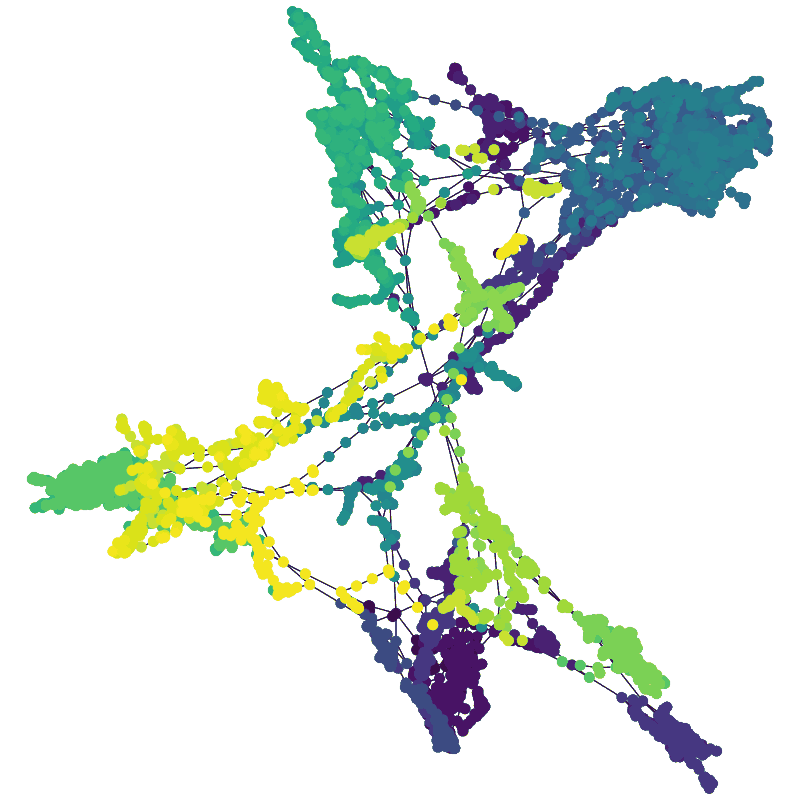
\includegraphics[width=0.27\columnwidth]{vis/USpowerGrid_CN-L-BFGS_2.png}} &
  \makecell{\textsf{BEST}\\[-0.2em]\includegraphics[width=0.27\columnwidth]{vis/opt_USpowerGrid_2.png}} \\

  \multicolumn{6}{c}{\large \textbf{\texttt{bcspwr10}} $(\abs{V}=5300, \abs{E}=8271, \text{density}=0.059\text{\%})$ \quad Figures are at 150 iterations.} \\
  \raisebox{-.5\height}{\includegraphics[width=0.55\columnwidth]{plot/bcspwr10_2.pdf}} &
  \makecell{\textsf{RAND-FR}\\[-0.2em]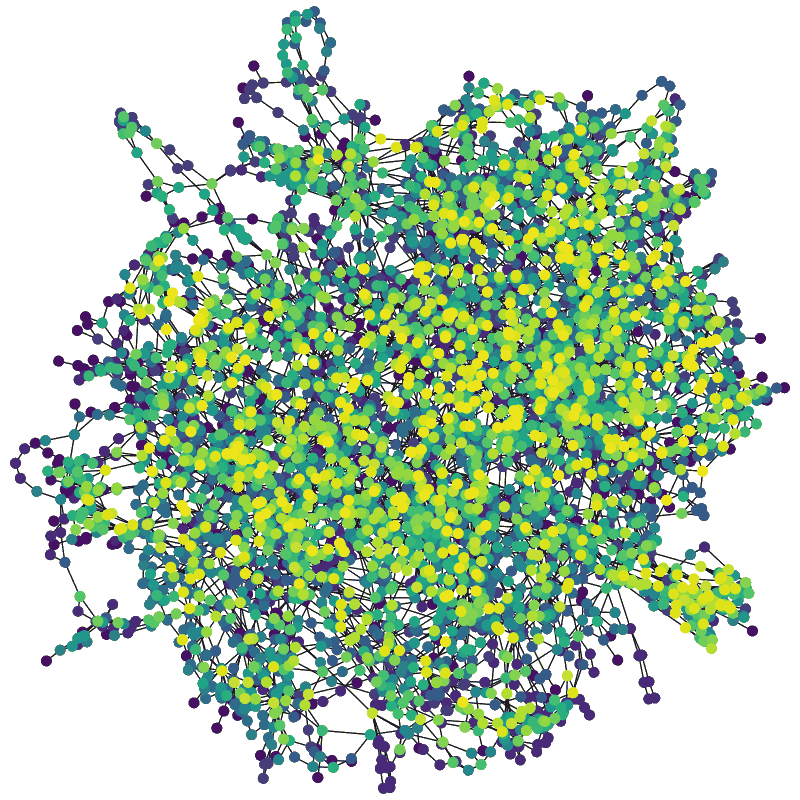
\includegraphics[width=0.27\columnwidth]{vis/bcspwr10_FR_2.png}} &
  \makecell{\textsf{\textbf{CN}-FR (proposed)}\\[-0.2em]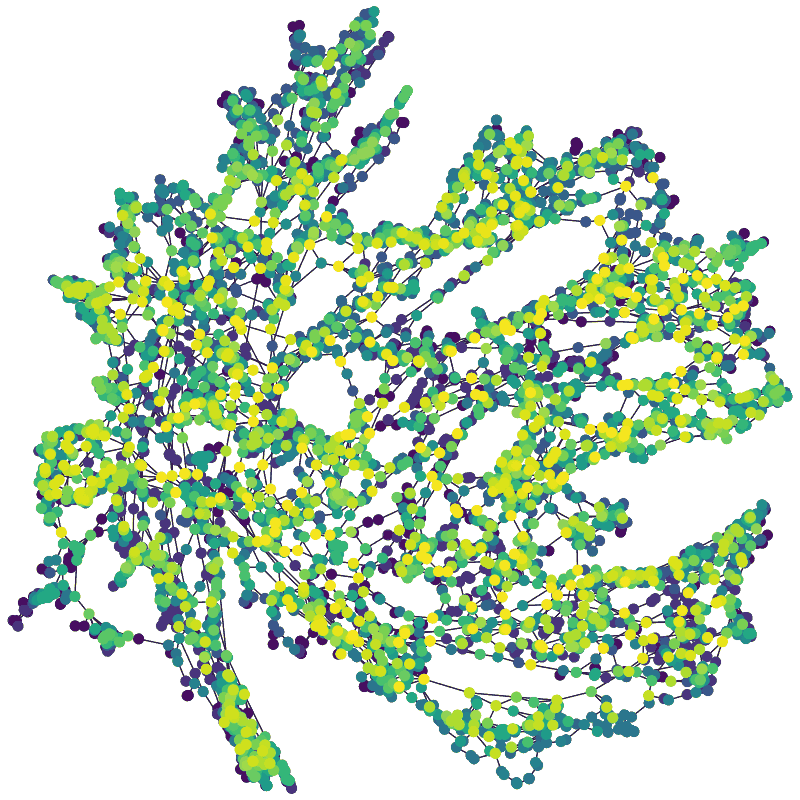
\includegraphics[width=0.27\columnwidth]{vis/bcspwr10_CN-FR_2.png}} &
  \makecell{\textsf{RAND-L-BFGS}\\[-0.2em]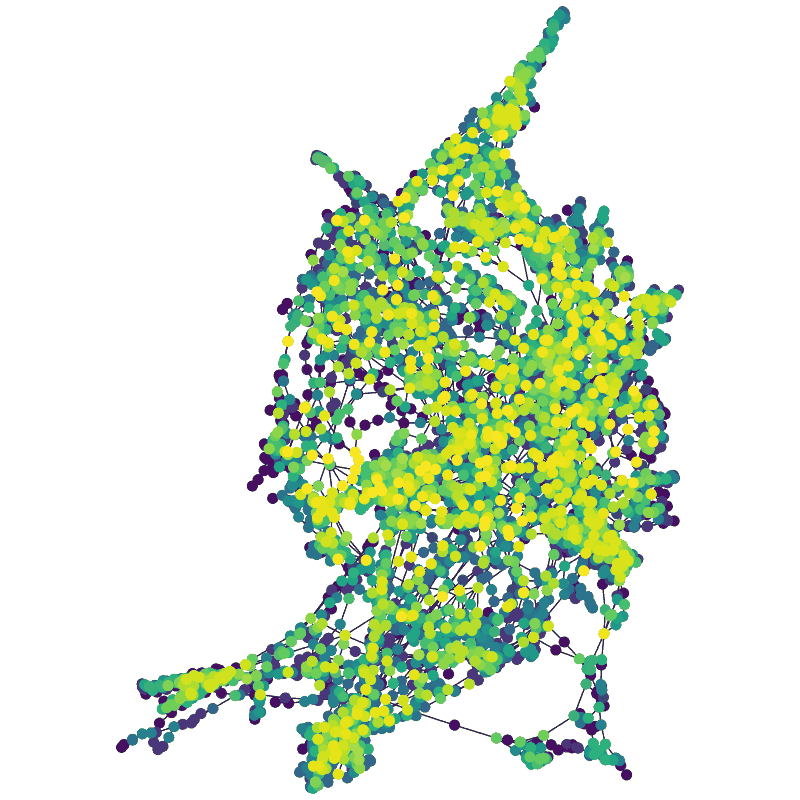
\includegraphics[width=0.27\columnwidth]{vis/bcspwr10_L-BFGS_2.png}} &
  \makecell{\textsf{\textbf{CN}-L-BFGS (proposed)}\\[-0.2em]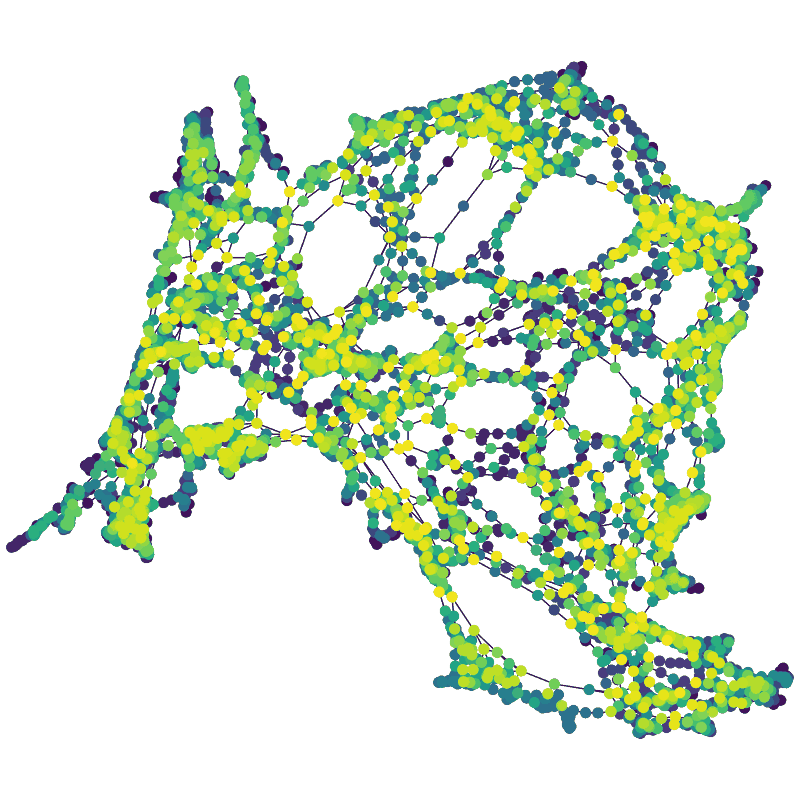
\includegraphics[width=0.27\columnwidth]{vis/bcspwr10_CN-L-BFGS_2.png}} &
  \makecell{\textsf{BEST}\\[-0.2em]\includegraphics[width=0.27\columnwidth]{vis/opt_bcspwr10_2.png}} \\

  \multicolumn{6}{c}{\large \textbf{\texttt{wiki-Vote}} $(\abs{V}=7066, \abs{E}=100736, \text{density}=0.404\text{\%})$ \quad Figures are at 150 iterations.} \\
  \raisebox{-.5\height}{\includegraphics[width=0.55\columnwidth]{plot/wiki-Vote_2.pdf}} &
  \makecell{\textsf{RAND-FR}\\[-0.2em]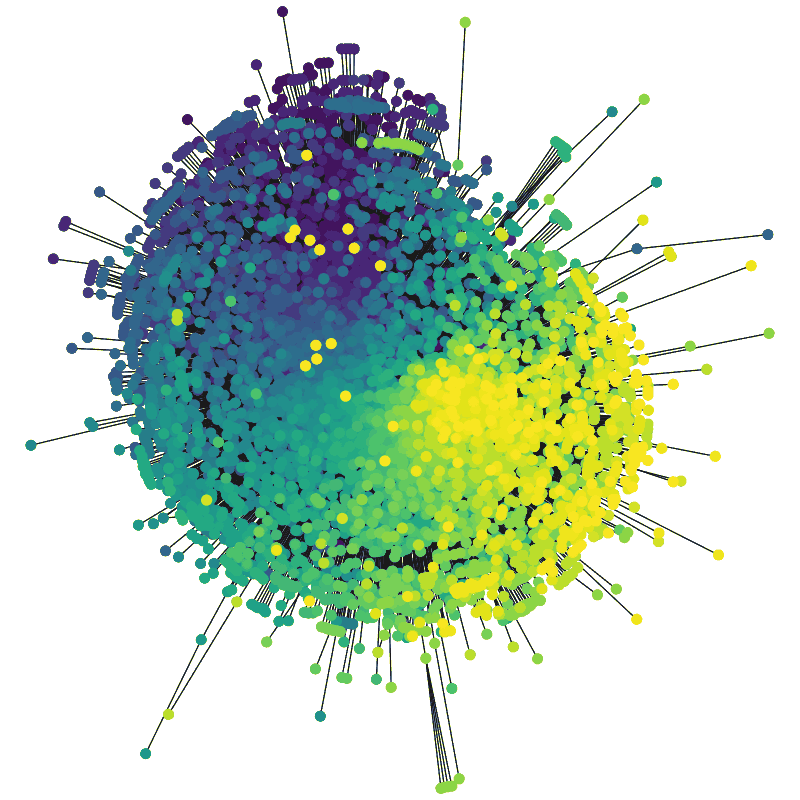
\includegraphics[width=0.27\columnwidth]{vis/wiki-Vote_FR_2.png}} &
  \makecell{\textsf{\textbf{CN}-FR (proposed)}\\[-0.2em]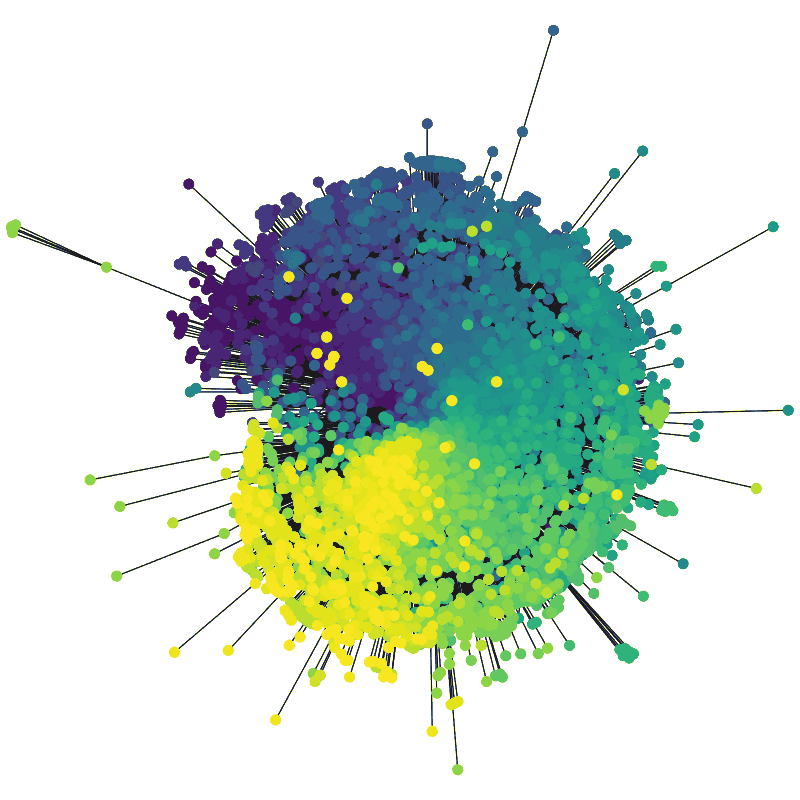
\includegraphics[width=0.27\columnwidth]{vis/wiki-Vote_CN-FR_2.png}} &
  \makecell{\textsf{RAND-L-BFGS}\\[-0.2em]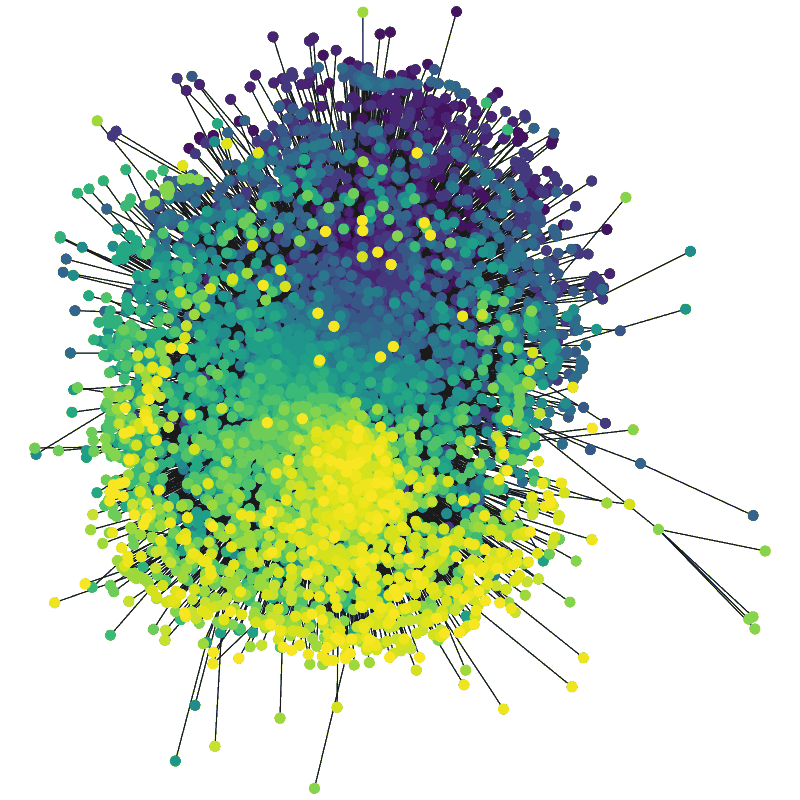
\includegraphics[width=0.27\columnwidth]{vis/wiki-Vote_L-BFGS_2.png}} &
  \makecell{\textsf{\textbf{CN}-L-BFGS (proposed)}\\[-0.2em]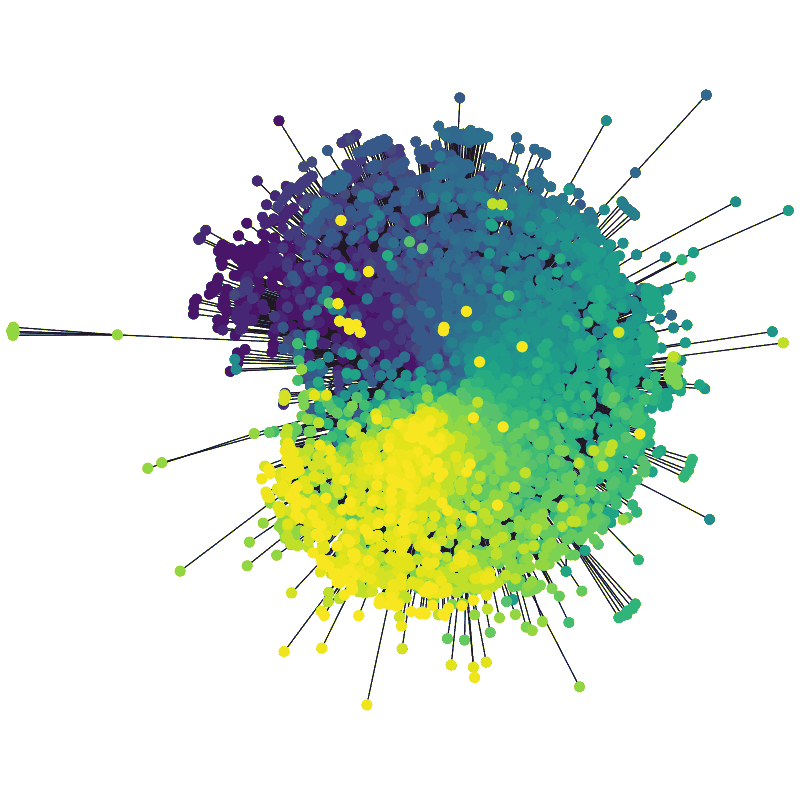
\includegraphics[width=0.27\columnwidth]{vis/wiki-Vote_CN-L-BFGS_2.png}} &
  \makecell{\textsf{BEST}\\[-0.2em]\includegraphics[width=0.27\columnwidth]{vis/opt_wiki-Vote_2.png}} \\
\end{tabular}
\end{document}
